\section{Астатизм первого порядка. PI регулятор}

Рассмотрим замкнутую системы с объектом управления, описываемым передаточной функцией:
\begin{equation}
    W(s) = \frac{3}{s^2 + 7.5s + 2}
\end{equation}
И регулятором, описываемым передаточной функцией:
\begin{equation}
   H(s) = k_p + \frac{k_i}{s}
\end{equation}
Запишем передаточную функцию замкнутой системы:
\begin{equation}
    W_{u\rightarrow y}(s) = \frac{W(s)H(s)}{1 + W(s)H(s)} = \frac{3(k_p + \frac{k_i}{s})}{s^2 + 7.5s + 2 + 3(k_p + \frac{k_i}{s})} = \frac{3k_p s + 3k_i}{s^3 + 7.5s^2 + (2 + 3k_p)s + 3k_i}
\end{equation}
Согласно следствию из критерия Гурвица для систем третьего порядка, система будет устойчива при:
\begin{equation}
    \begin{cases}
        7.5 > 0 \\ 
        2 + 3k_p > 0 \\ 
        3k_i > 0 \\ 
        7.5 \cdot 2 > 3k_i \\
    \end{cases}
    \Rightarrow
    \begin{cases}
        k_p > -\frac{2}{3} \\ 
        k_i > 0 \\ 
        k_i < 5
    \end{cases}
\end{equation}
Найдем передаточную функцию по ошибке:
\begin{multline}
    W_{u\rightarrow e}(s) = \frac{1}{1 + W(s)H(s)} = \frac{1}{1 + \frac{3}{s^2 + 7.5s + 2}( k_p + \frac{k_i}{s})} = \frac{s^3 + 7.5s^2 + 2s}{s^3 + 7.5s^2 + (2 + 3k_p)s + 3k_i} 
\end{multline}

\subsection{Система с линейно возрастающим входным воздействием}
Рассмотрим систему с линейно возрастающим входным воздействием:
\begin{equation}
    u(t) = Vt
\end{equation}
Найдем образ Лапласа входного воздействия:
\begin{equation}
    L\{u\} = \frac{V}{s^2}
\end{equation}
Найдем образ Лапласа выходного сигнала:
\begin{equation}
    Y = W_{u\rightarrow y}(s)L\{u\} = \frac{3k_p s + 3k_i}{s^3 + 7.5s^2 + (2 + 3k_p)s + 3k_i}\frac{V}{s^2}
\end{equation}
И образ Лапласа ошибки:
\begin{equation}
    E = W_{u\rightarrow e}(s)L\{u\} = \frac{s^3 + 7.5s^2 + 2s}{s^3 + 7.5s^2 + (2 + 3k_p)s + 3k_i}\frac{V}{s^2}
\end{equation}
Согласно теореме о конечном значении, установившееся значение ошибки равно:
\begin{equation}
    e_{\text{set}} = \lim_{s \to 0} sE = \lim_{s \to 0} \frac{V(s^2 + 7.5s + 2)}{s^3 + 7.5s^2 + (2 + 3k_p)s + 3k_i} = \frac{2V}{3k_i}
\end{equation}
В качестве значений коэффициентов возьмем:
\begin{table}[ht!]
    \centering
    \begin{tabular}{|c|c|c|}
        \hline
        $k_p$ & $k_i$  \\
        \hline
        1 & 0.1 \\
        5 & 0.3 \\
        10 & 0.5 \\
        \hline
    \end{tabular}
    \caption{Значения коэффициентов для PI регулятора}
    \label{tab:task5}
\end{table}

Для всех возможных комбинаций коэффициентов промоделируем систему. 

При $k_p = 1$ графики выходного сигнала и ошибки приведены
на рис. \ref{fig:task5_out1} и \ref{fig:task5_error1} соответственно.

\begin{figure}[ht!]
    \centering
    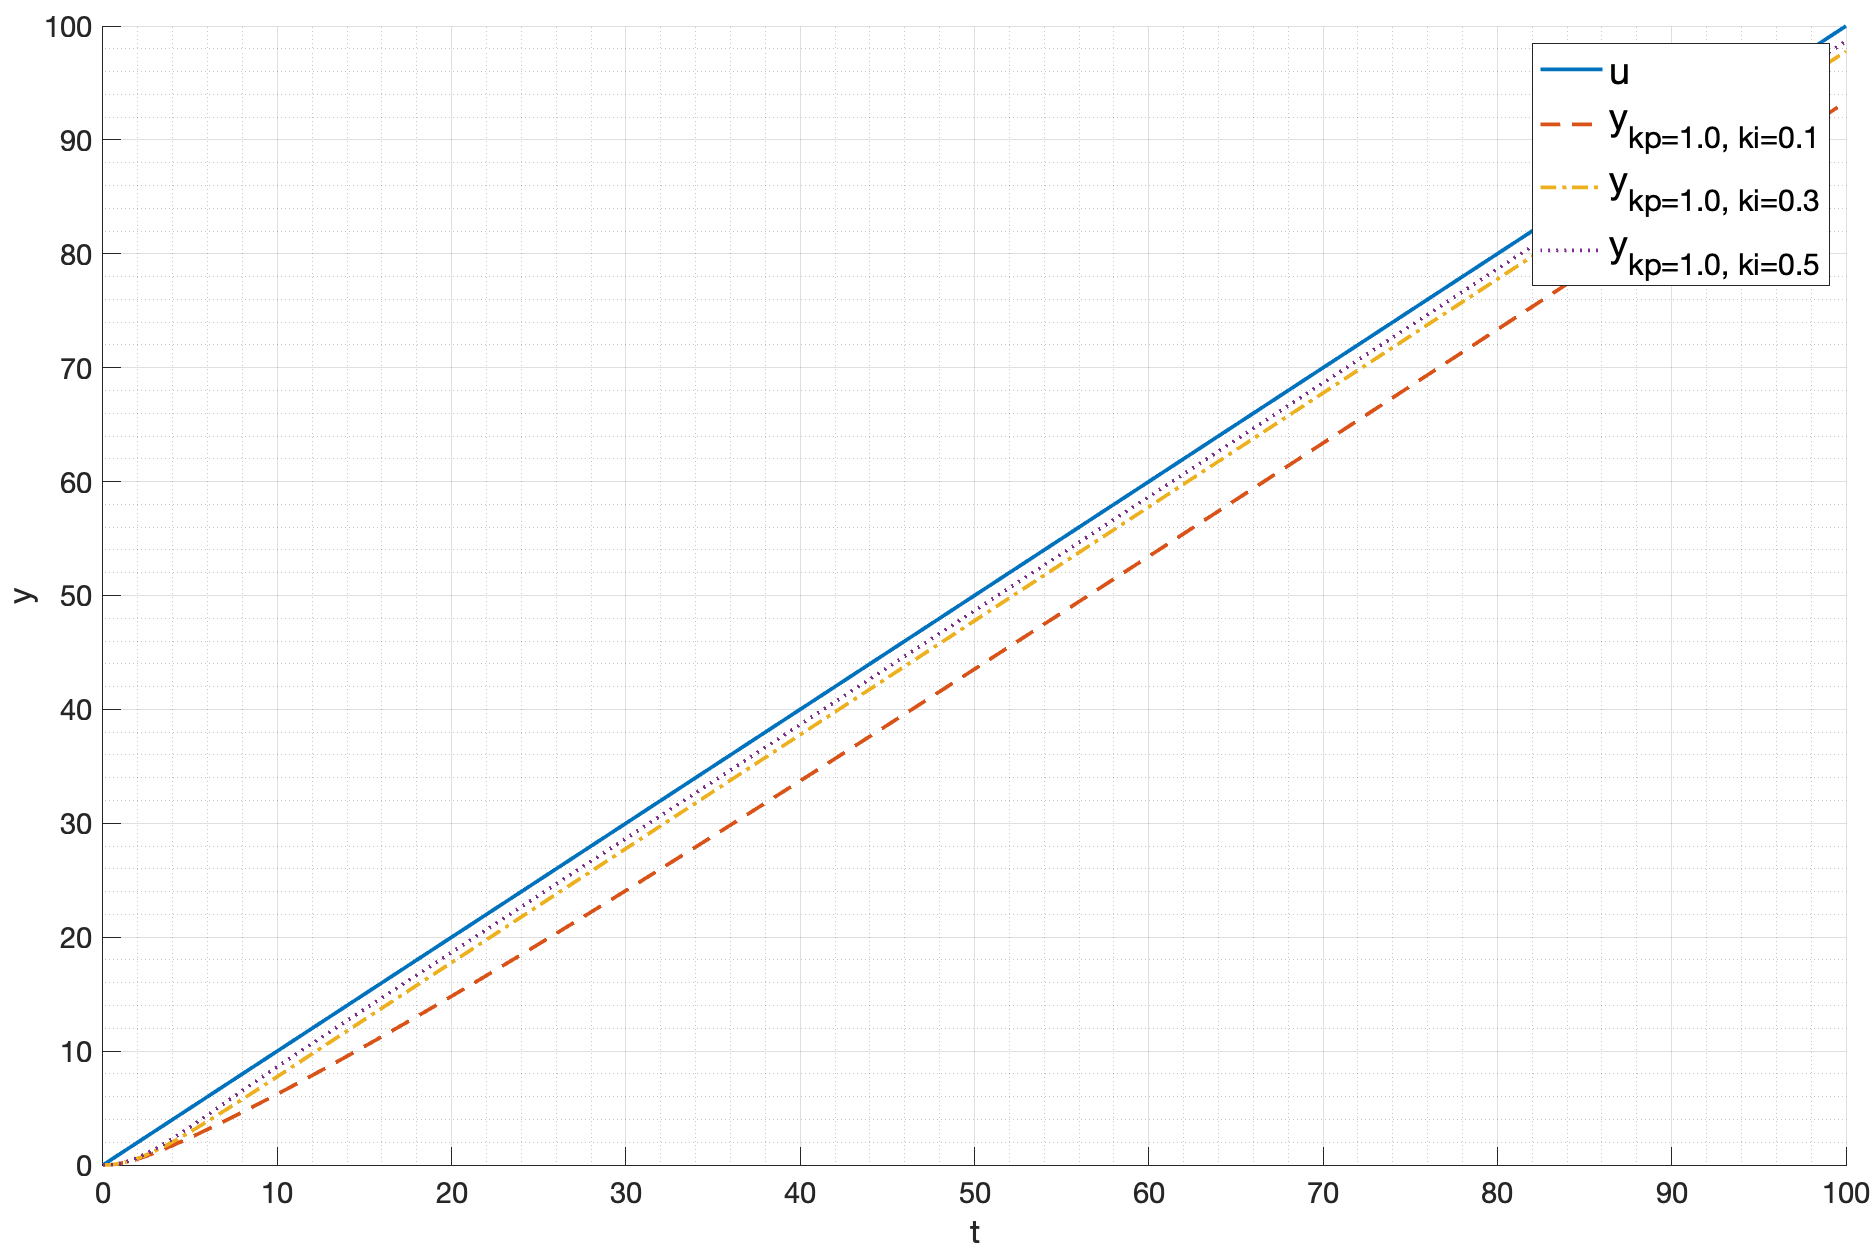
\includegraphics[width=\textwidth]{media/plots/task5_out_kp_1.0_1.png}
    \caption{График выходного сигнала при $k_p = 1$}
    \label{fig:task5_out1}
\end{figure}

\begin{figure}[ht!]
    \centering
    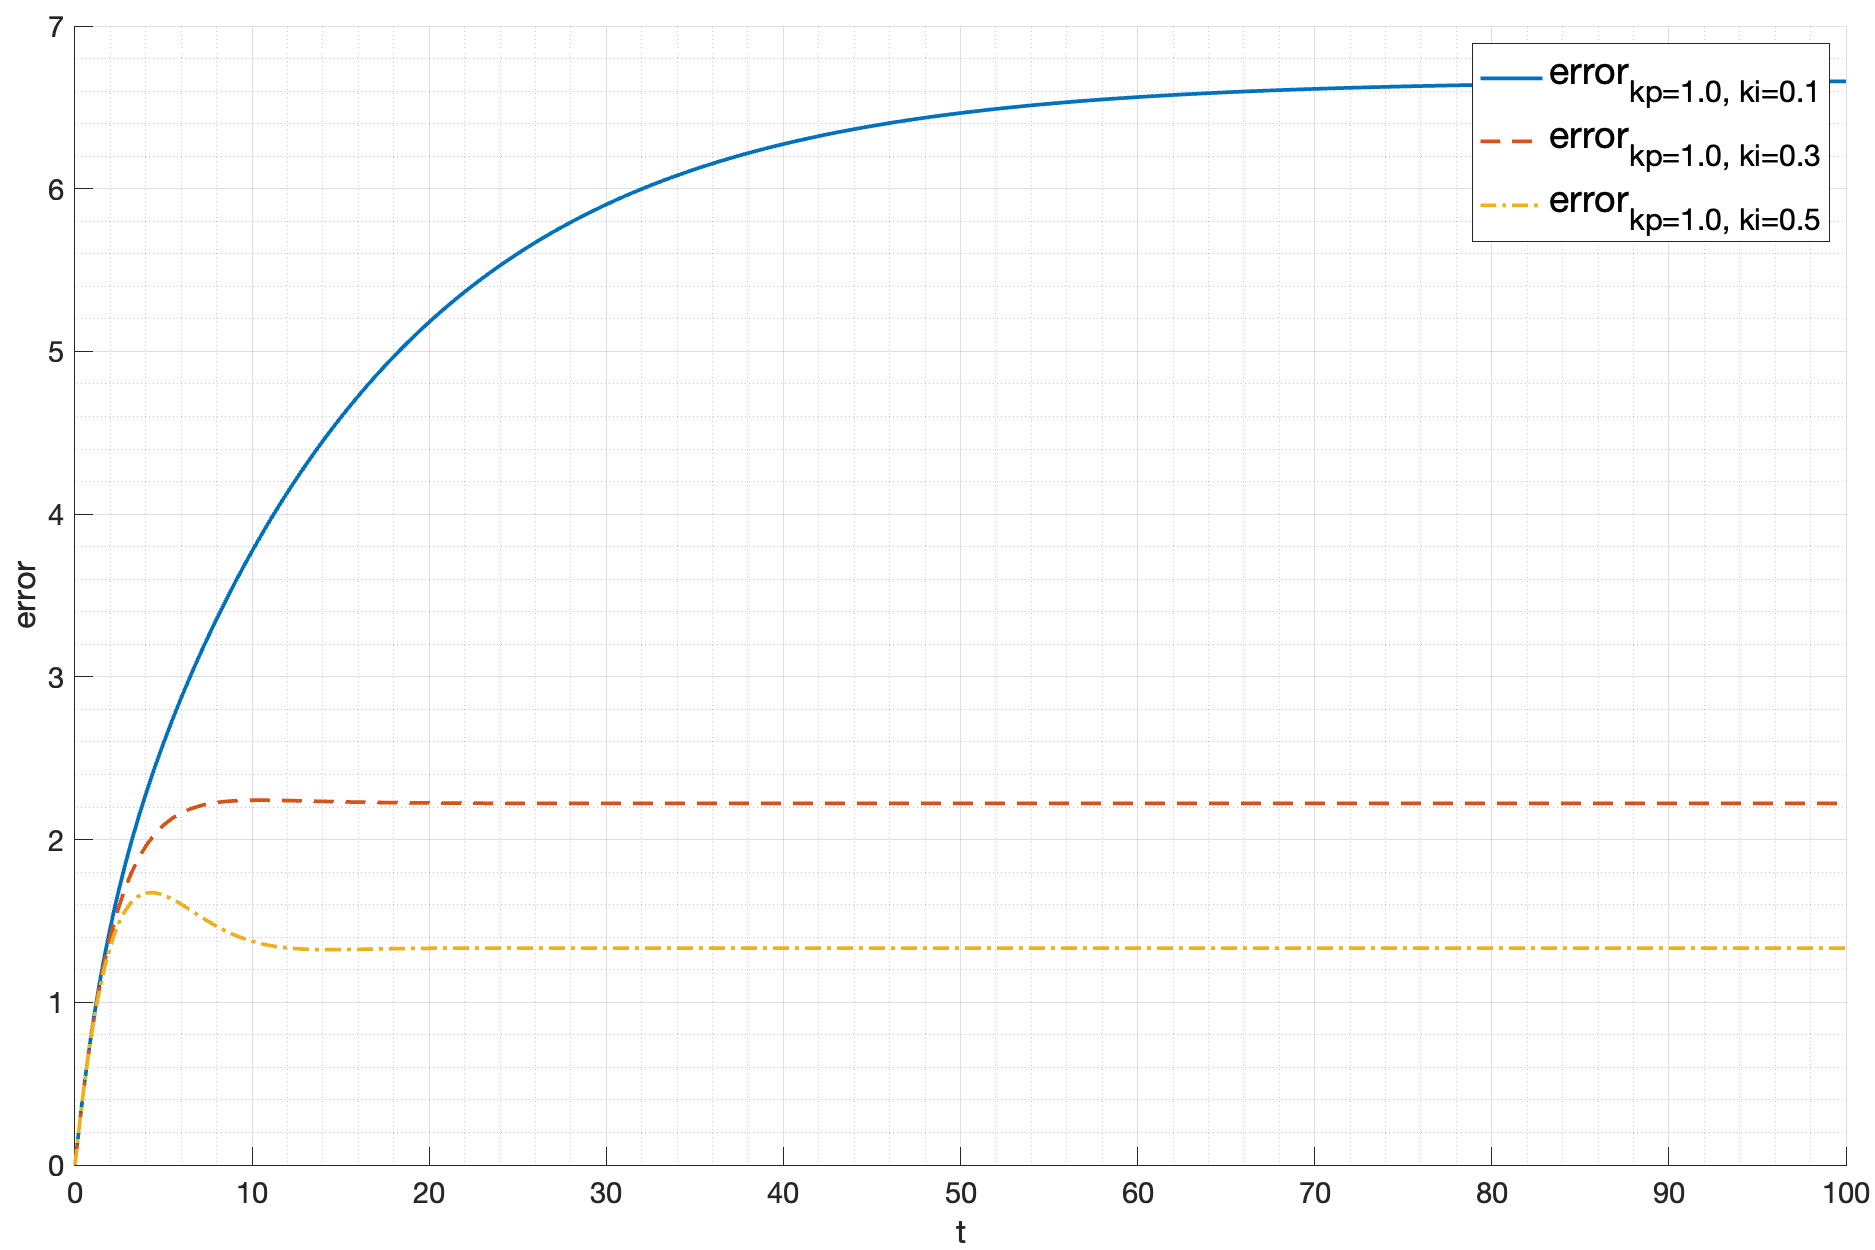
\includegraphics[width=\textwidth]{media/plots/task5_error_kp_1.0_1.png}
    \caption{График ошибки при $k_p = 1$}
    \label{fig:task5_error1}
\end{figure}

При $k_p = 5$ графики выходного сигнала и ошибки приведены
на рис. \ref{fig:task5_out2} и \ref{fig:task5_error2} соответственно.

\begin{figure}[ht!]
    \centering
    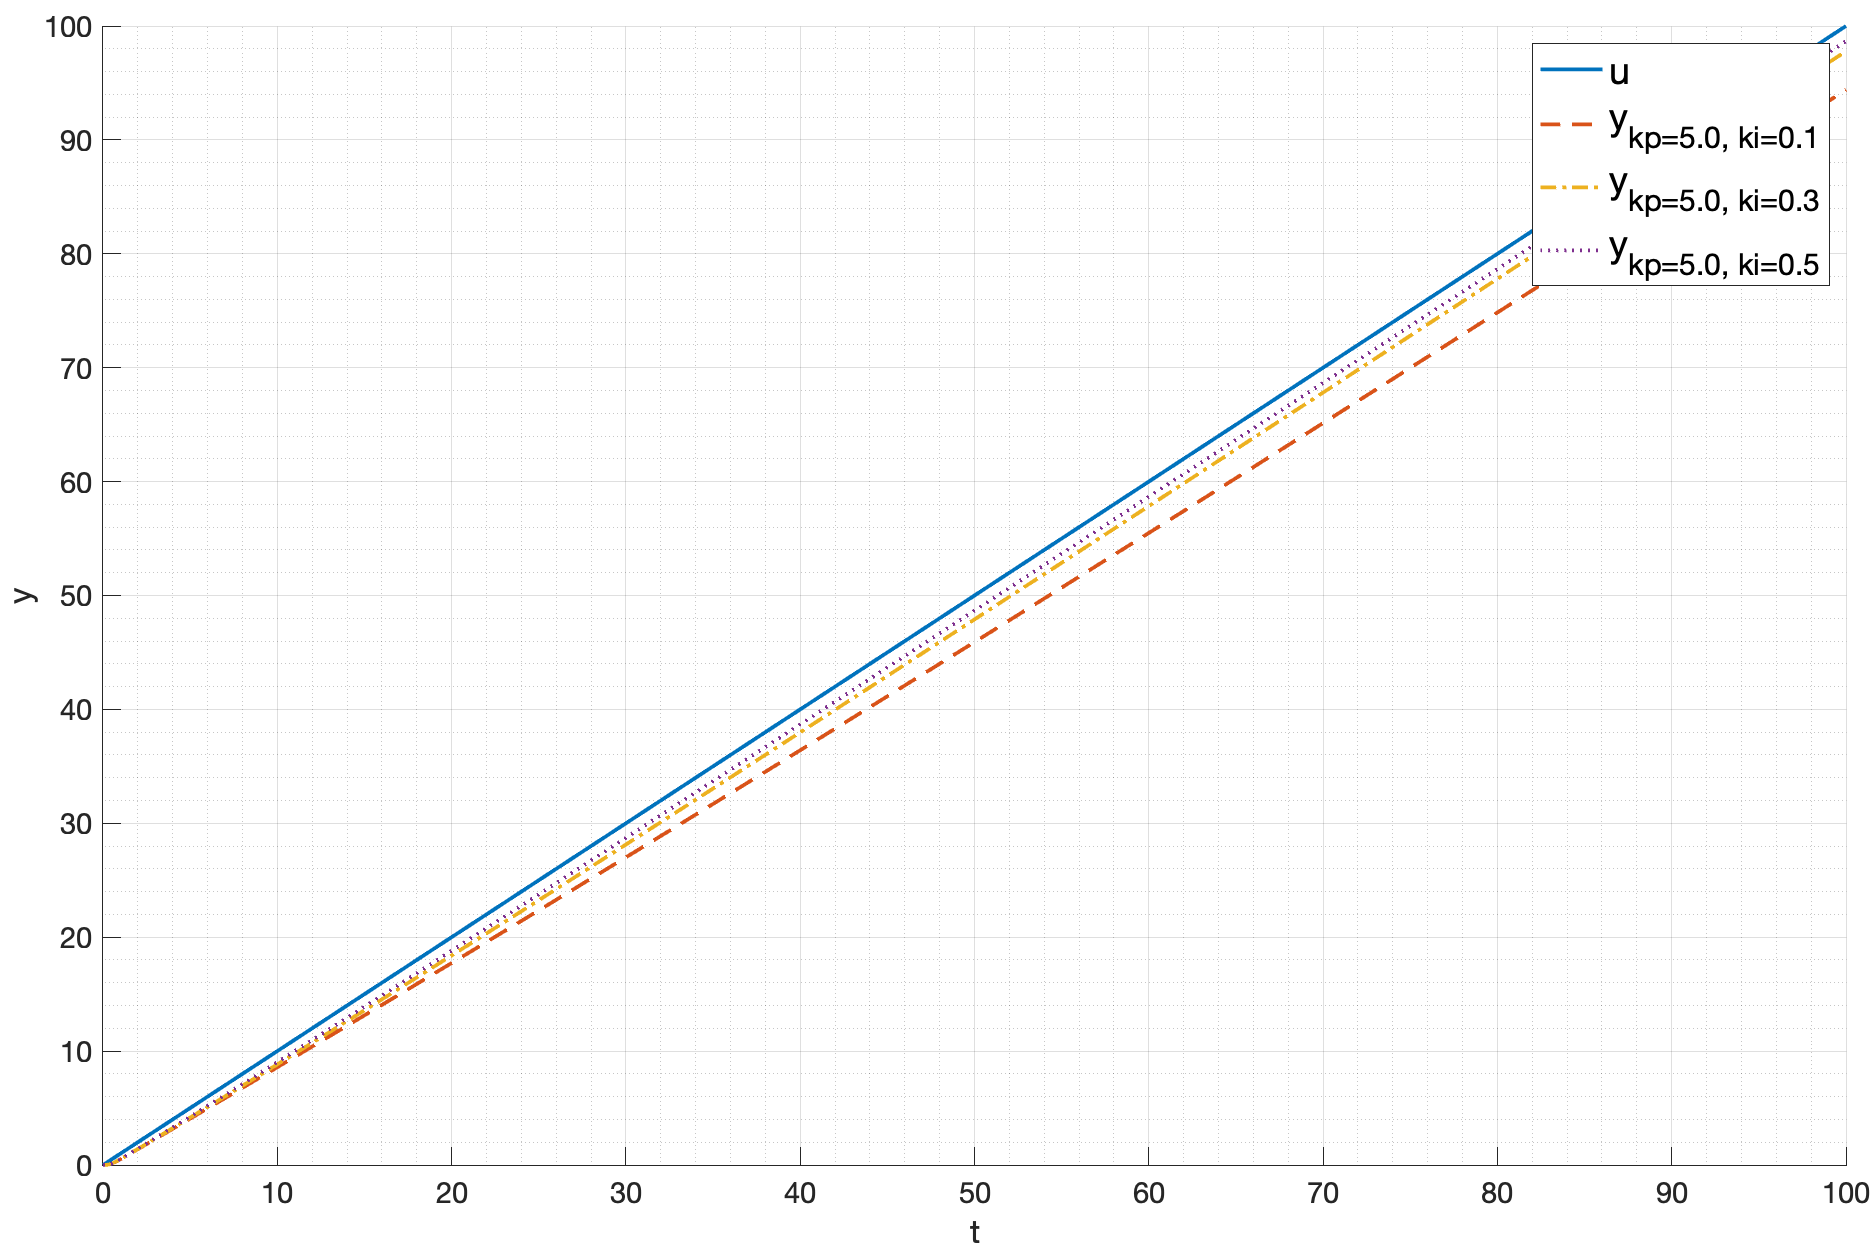
\includegraphics[width=\textwidth]{media/plots/task5_out_kp_5.0_1.png}
    \caption{График выходного сигнала при $k_p = 5$}
    \label{fig:task5_out2}
\end{figure}

\begin{figure}[ht!]
    \centering
    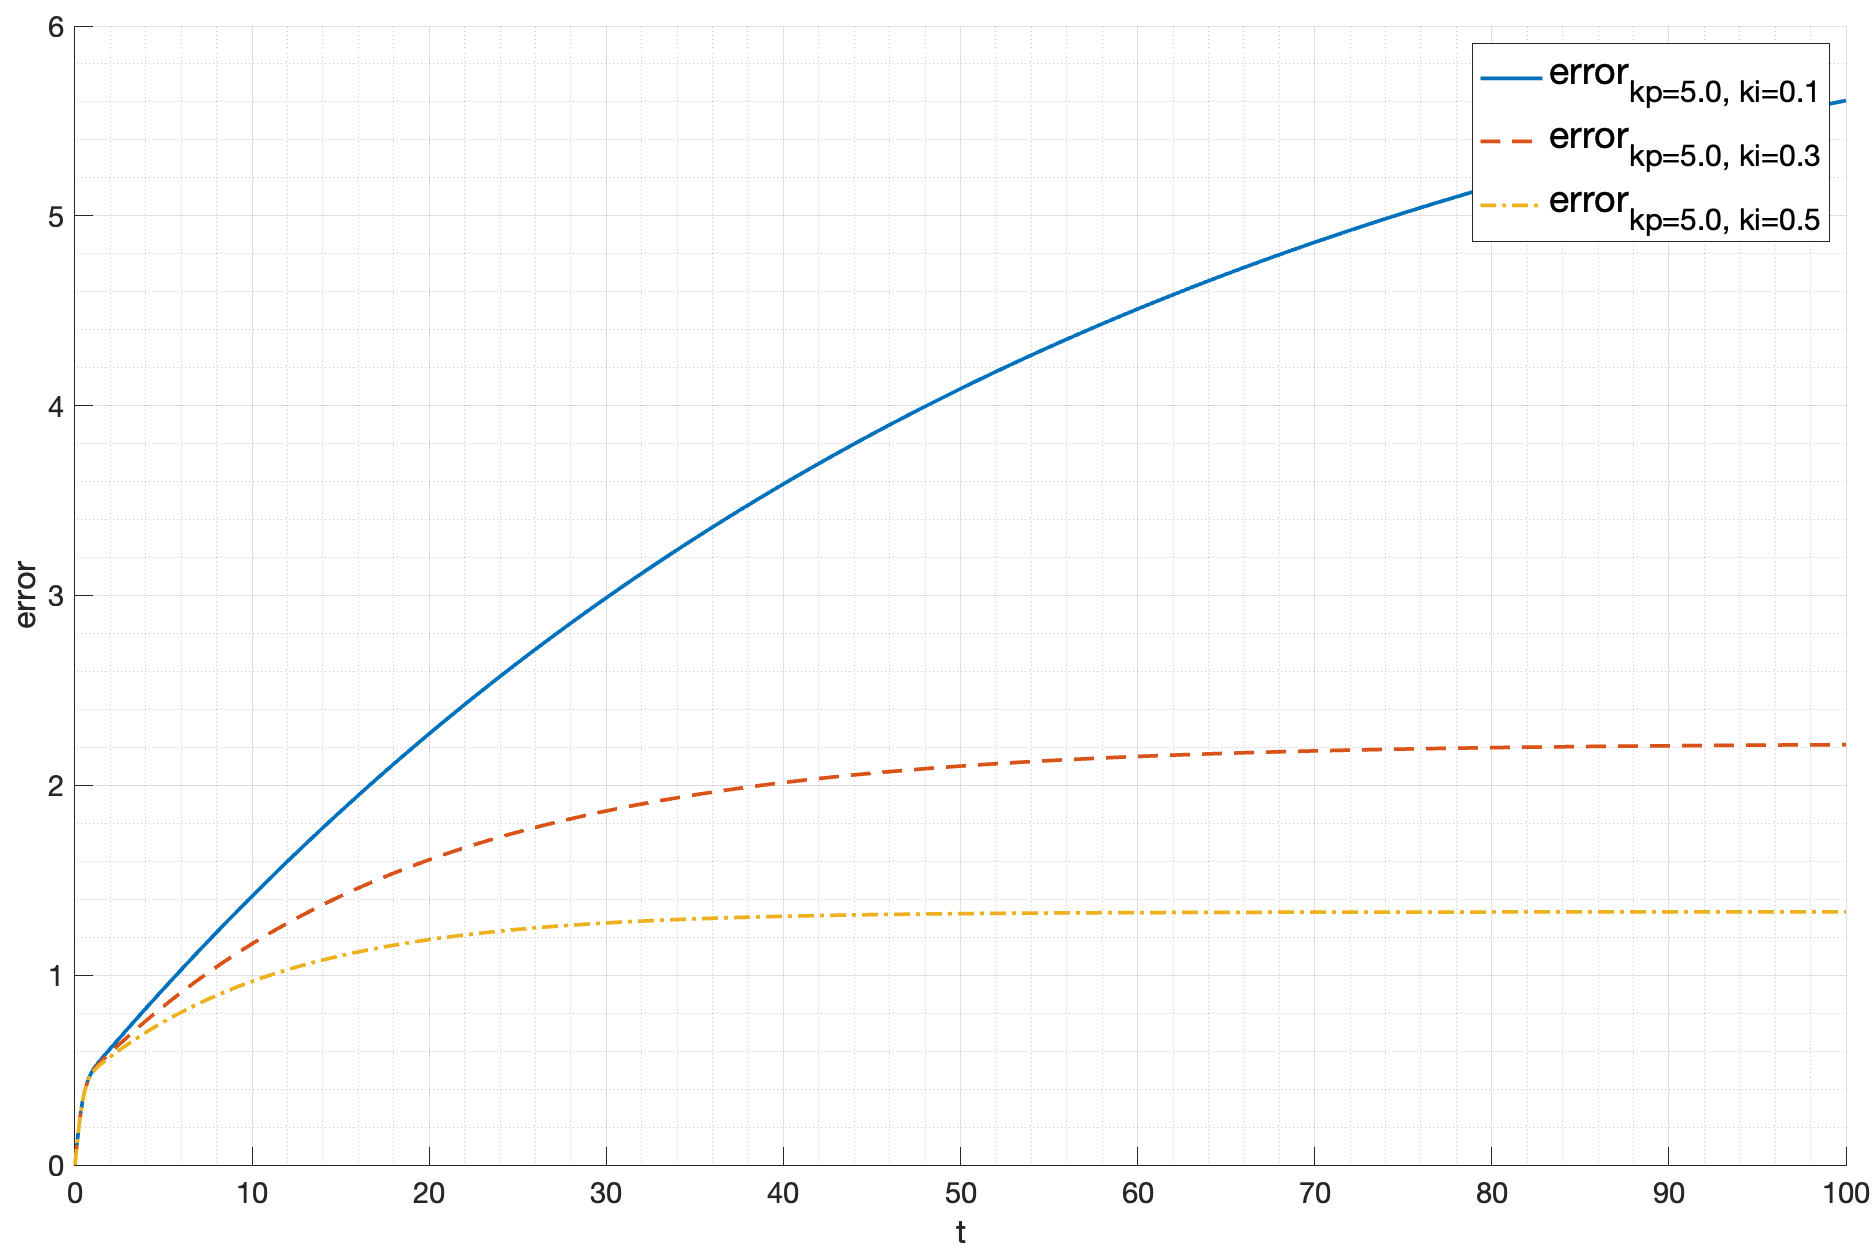
\includegraphics[width=\textwidth]{media/plots/task5_error_kp_5.0_1.png}
    \caption{График ошибки при $k_p = 5$}
    \label{fig:task5_error2}
\end{figure}

При $k_p = 10$ графики выходного сигнала и ошибки приведены
на рис. \ref{fig:task5_out3} и \ref{fig:task5_error3} соответственно.

\begin{figure}[ht!]
    \centering
    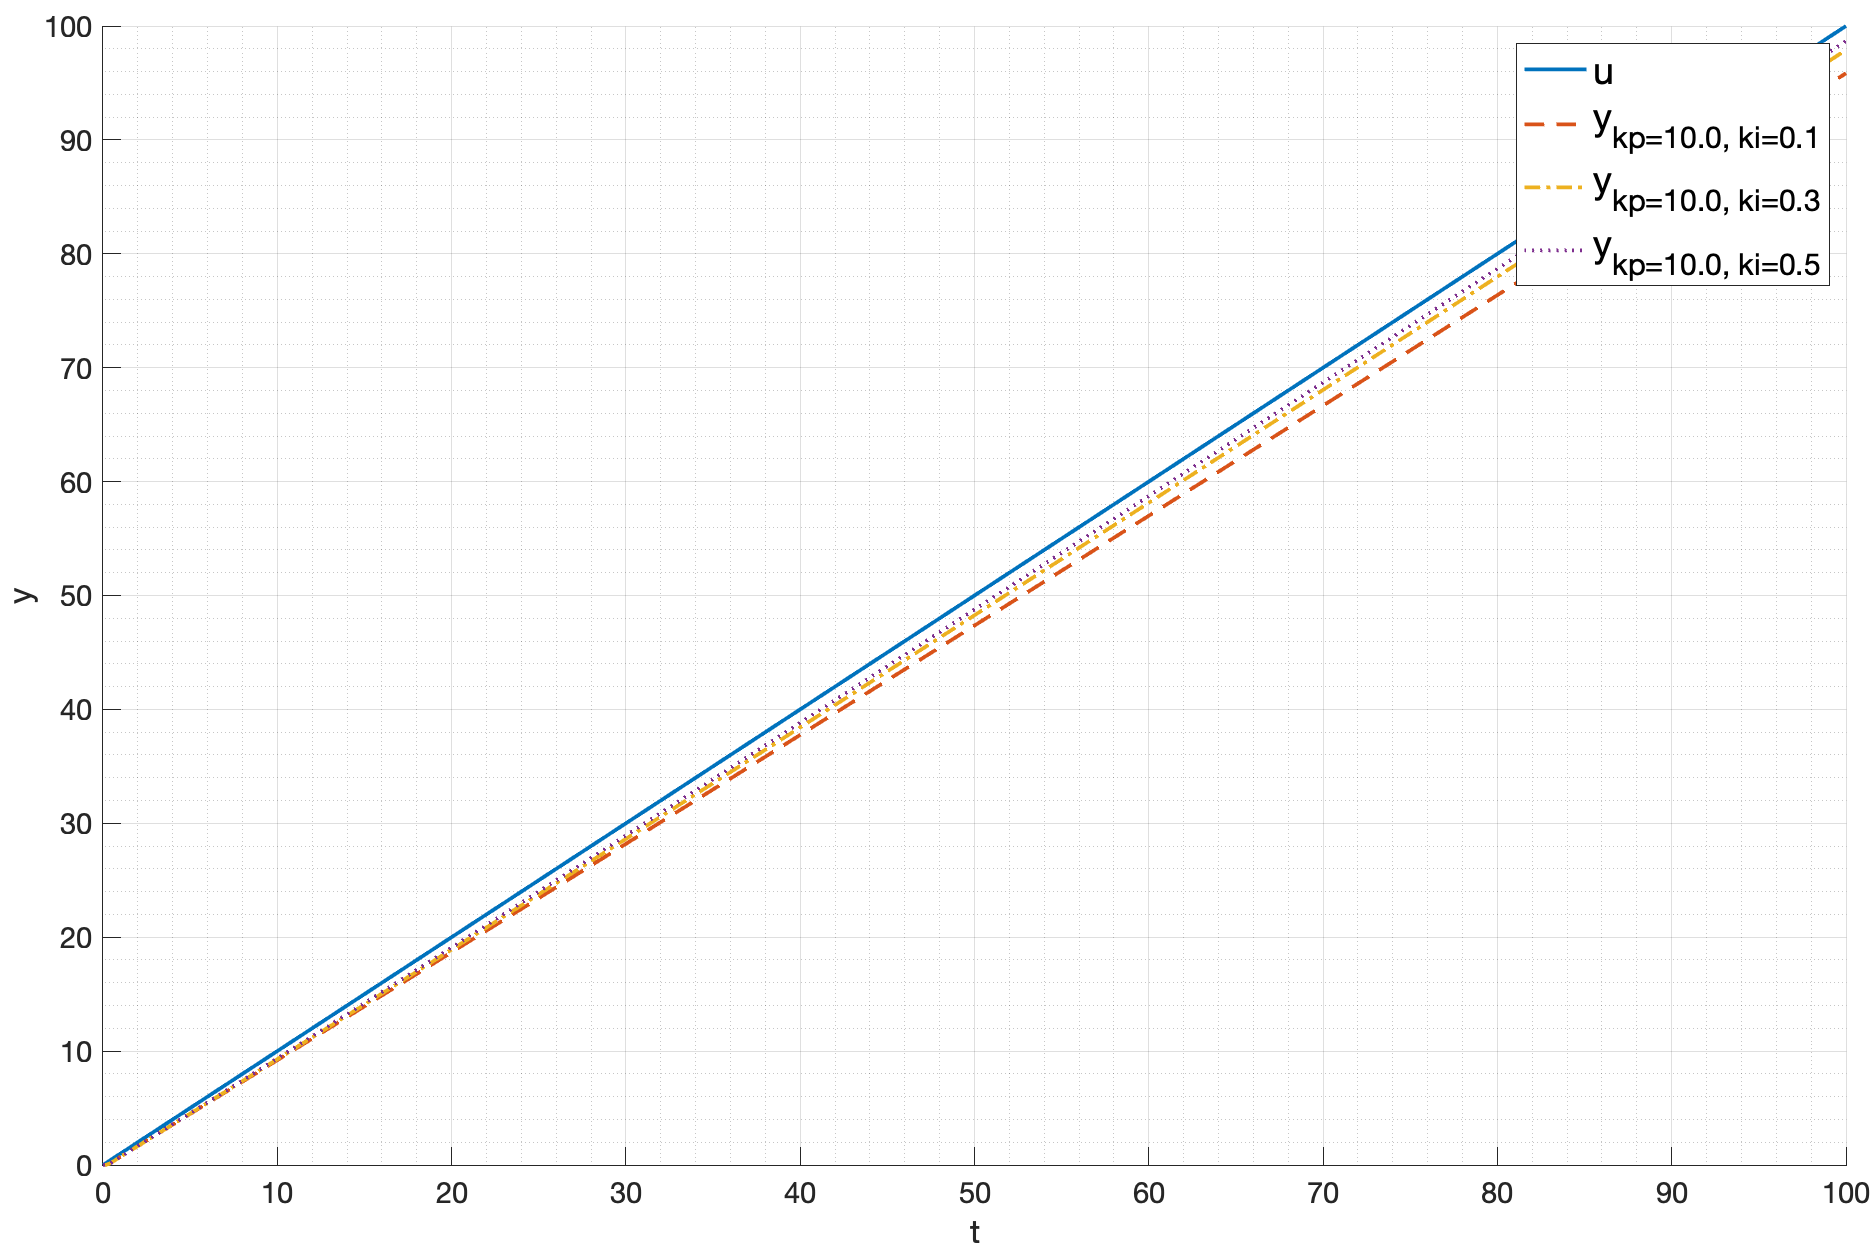
\includegraphics[width=\textwidth]{media/plots/task5_out_kp_10.0_1.png}
    \caption{График выходного сигнала при $k_p = 10$}
    \label{fig:task5_out3}
\end{figure}

\begin{figure}[ht!]
    \centering
    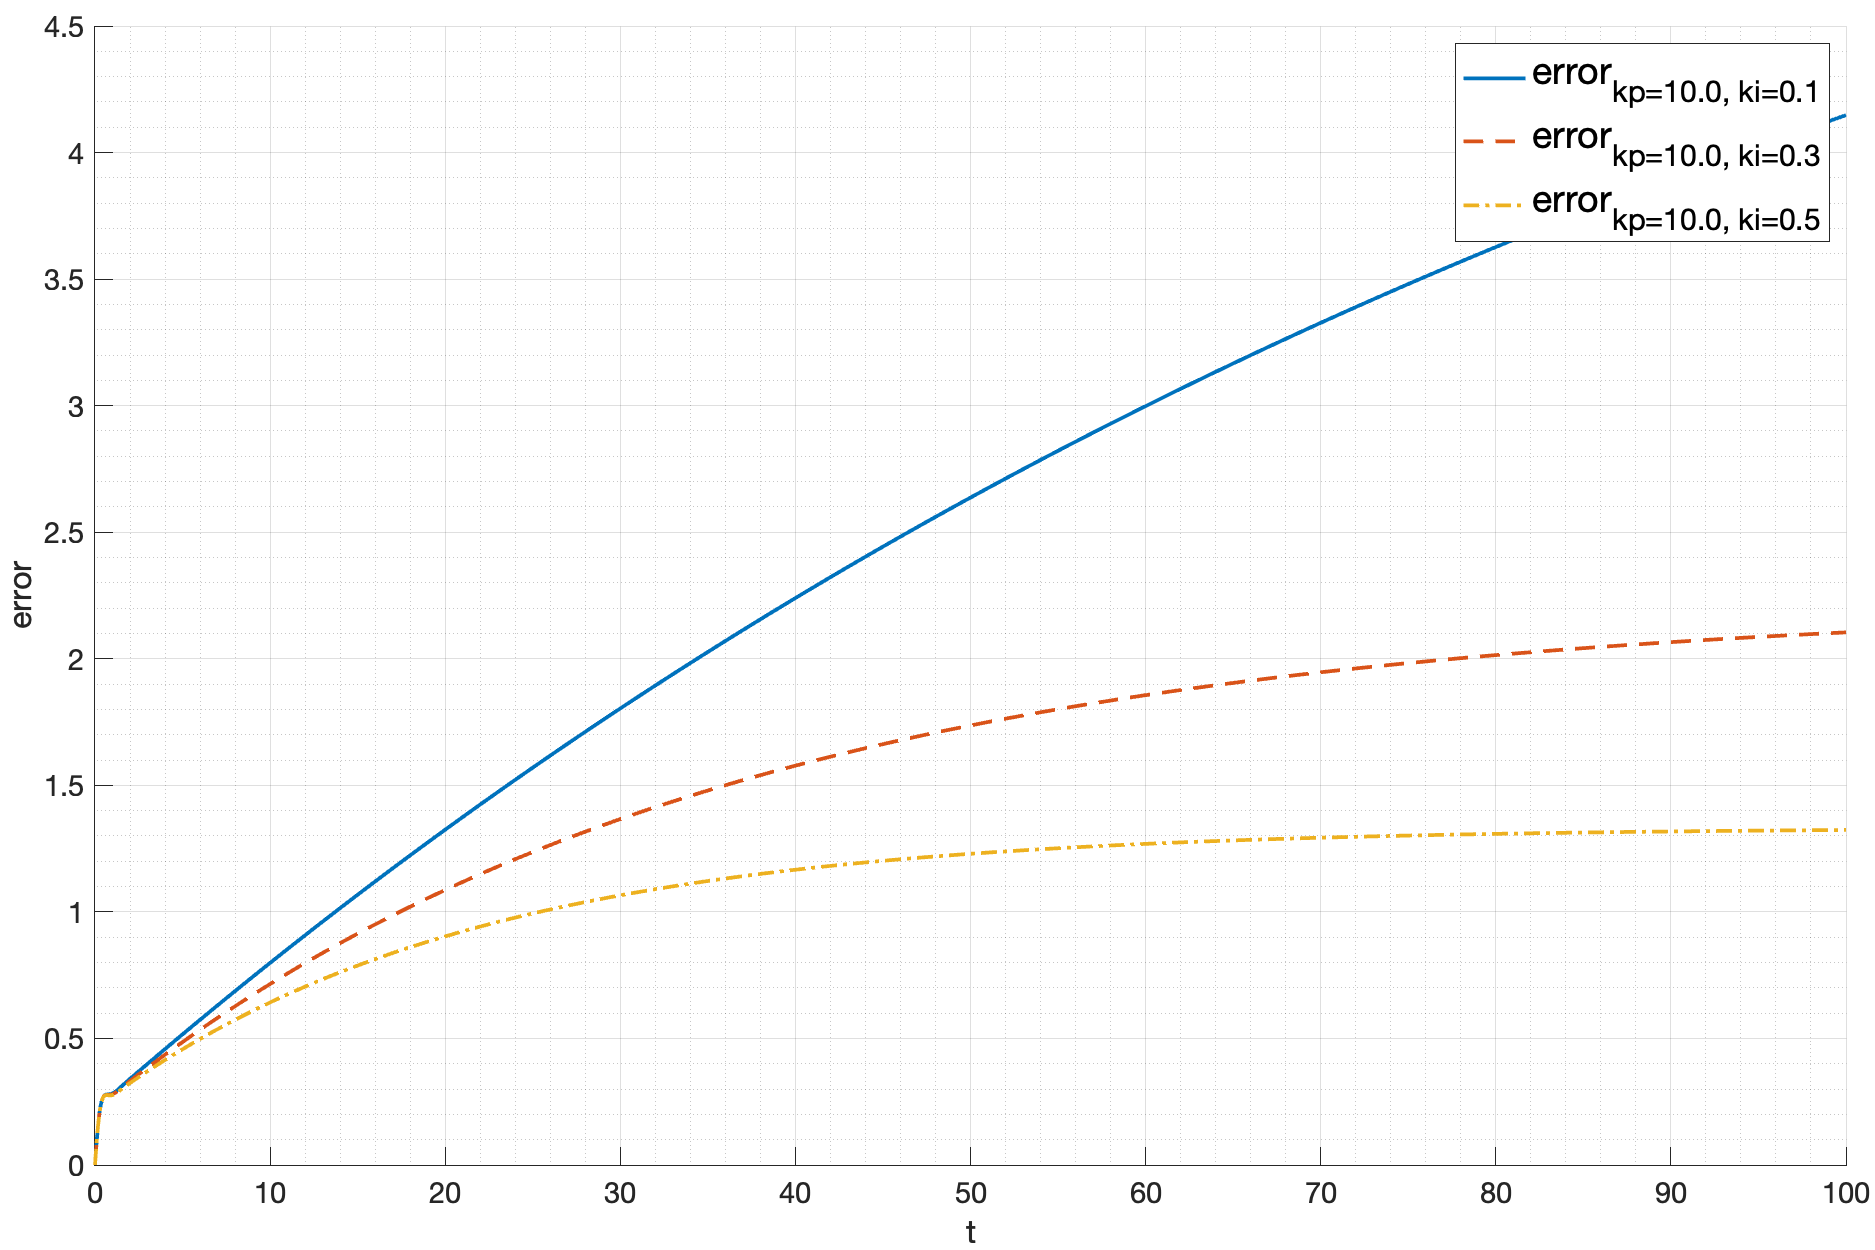
\includegraphics[width=\textwidth]{media/plots/task5_error_kp_10.0_1.png}
    \caption{График ошибки при $k_p = 10$}
    \label{fig:task5_error3}
\end{figure}

Во всех случаях система сходится к заданному значению с постоянной ошибкой, равной теоретическому значению.
Коэффициенты $k_p$ и $k_i$ влияют на скорость сходимости системы и на величину ошибки. 
При увеличении коэффициента $k_p$ система быстрее сходится к установившемуся значению,
при увеличении коэффициента $k_i$ уменьшается ошибка.

\FloatBarrier
\subsection{Слежение за гармоническим воздействием}

Рассмотрим систему с гармоническим входным воздействием:
\begin{equation}
    u(t) = A\sin(\omega t)
\end{equation}

При $k_p = 1$ графики выходного сигнала и ошибки приведены
на рис. \ref{fig:task5_out4} и \ref{fig:task5_error4} соответственно.

\begin{figure}[ht!]
    \centering
    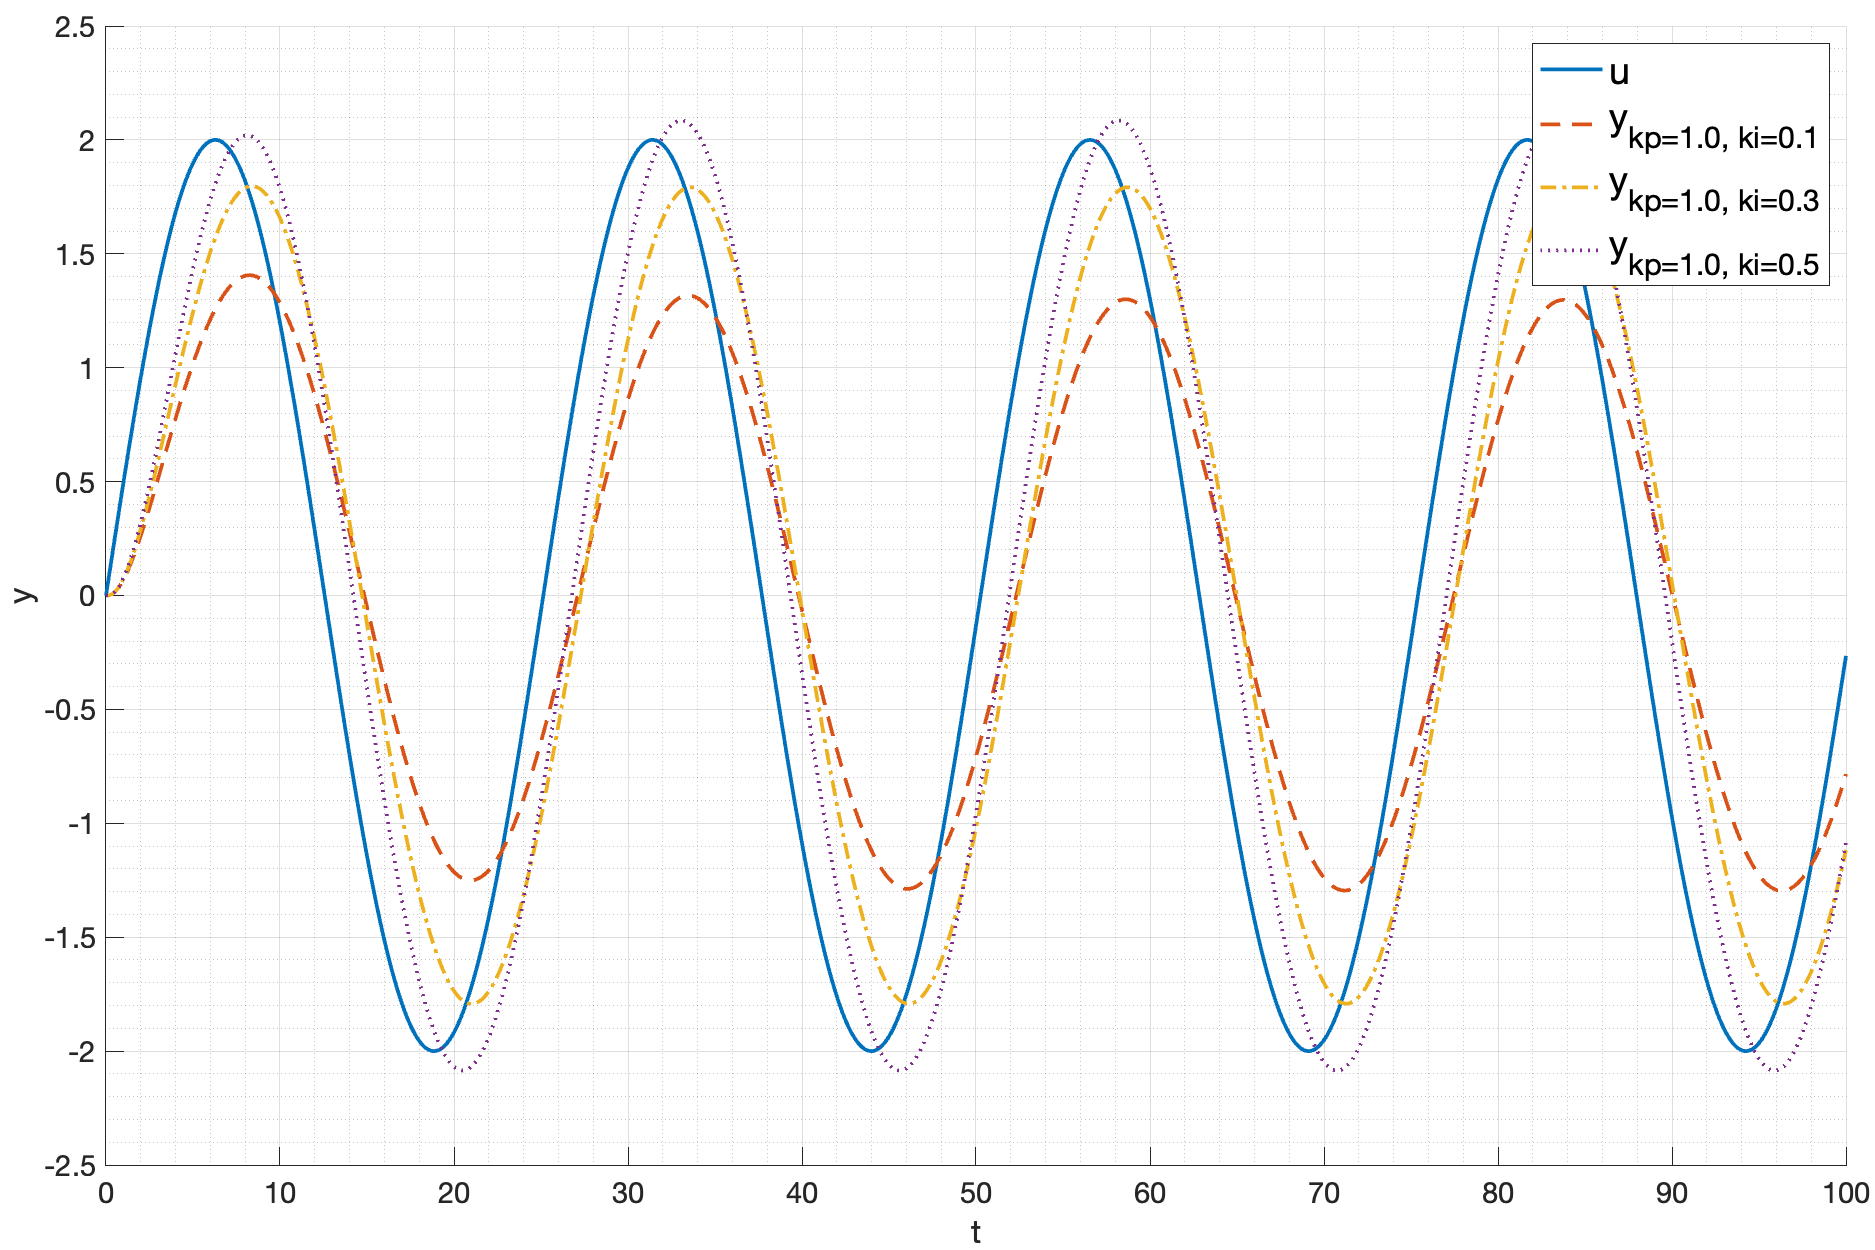
\includegraphics[width=\textwidth]{media/plots/task5_out_kp_1.0_2.png}
    \caption{График выходного сигнала при $k_p = 1$}
    \label{fig:task5_out4}
\end{figure}

\begin{figure}[ht!]
    \centering
    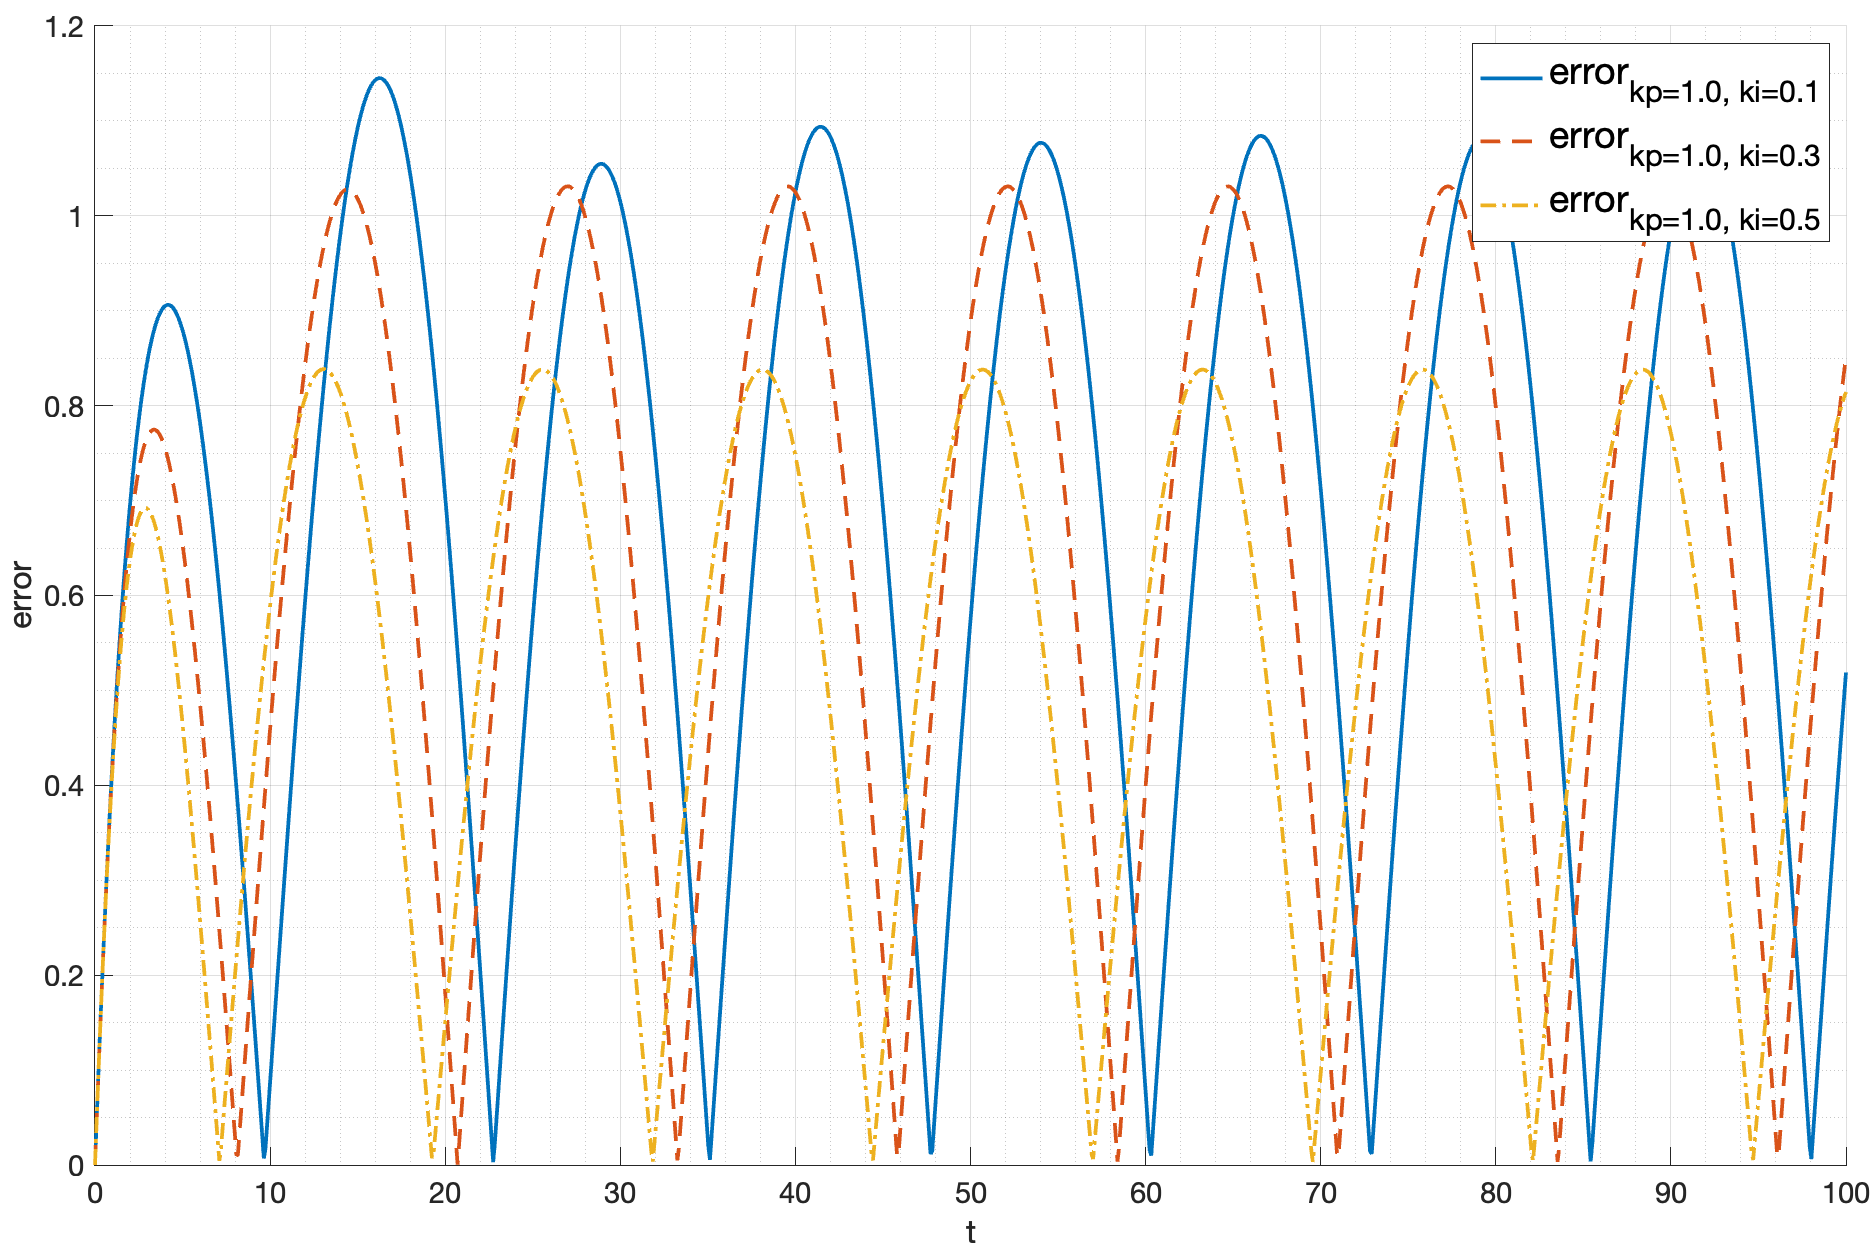
\includegraphics[width=\textwidth]{media/plots/task5_error_kp_1.0_2.png}
    \caption{График ошибки при $k_p = 1$}
    \label{fig:task5_error4}
\end{figure}

При $k_p = 5$ графики выходного сигнала и ошибки приведены
на рис. \ref{fig:task5_out5} и \ref{fig:task5_error5} соответственно.

\begin{figure}[ht!]
    \centering
    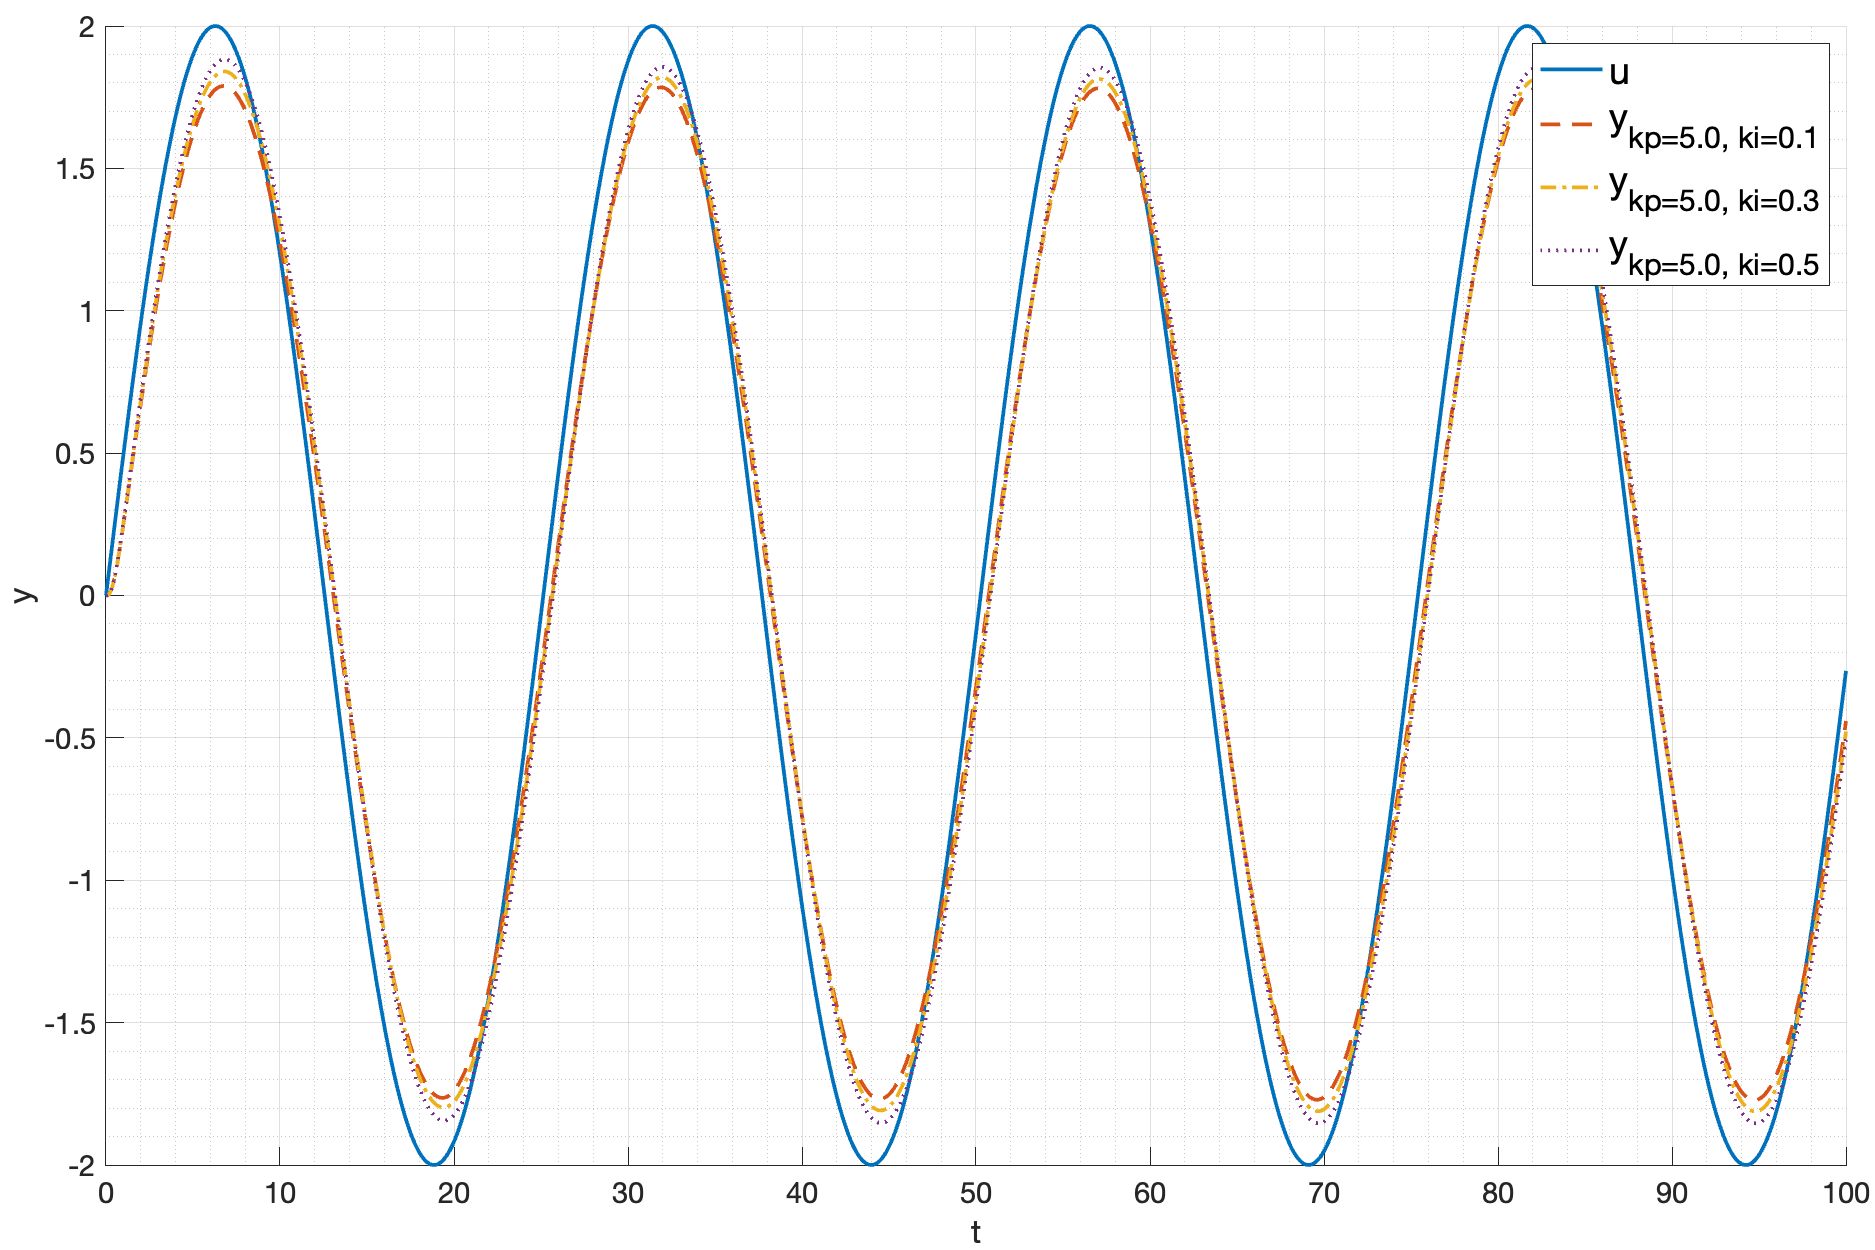
\includegraphics[width=\textwidth]{media/plots/task5_out_kp_5.0_2.png}
    \caption{График выходного сигнала при $k_p = 5$}
    \label{fig:task5_out5}
\end{figure}

\begin{figure}[ht!]
    \centering
    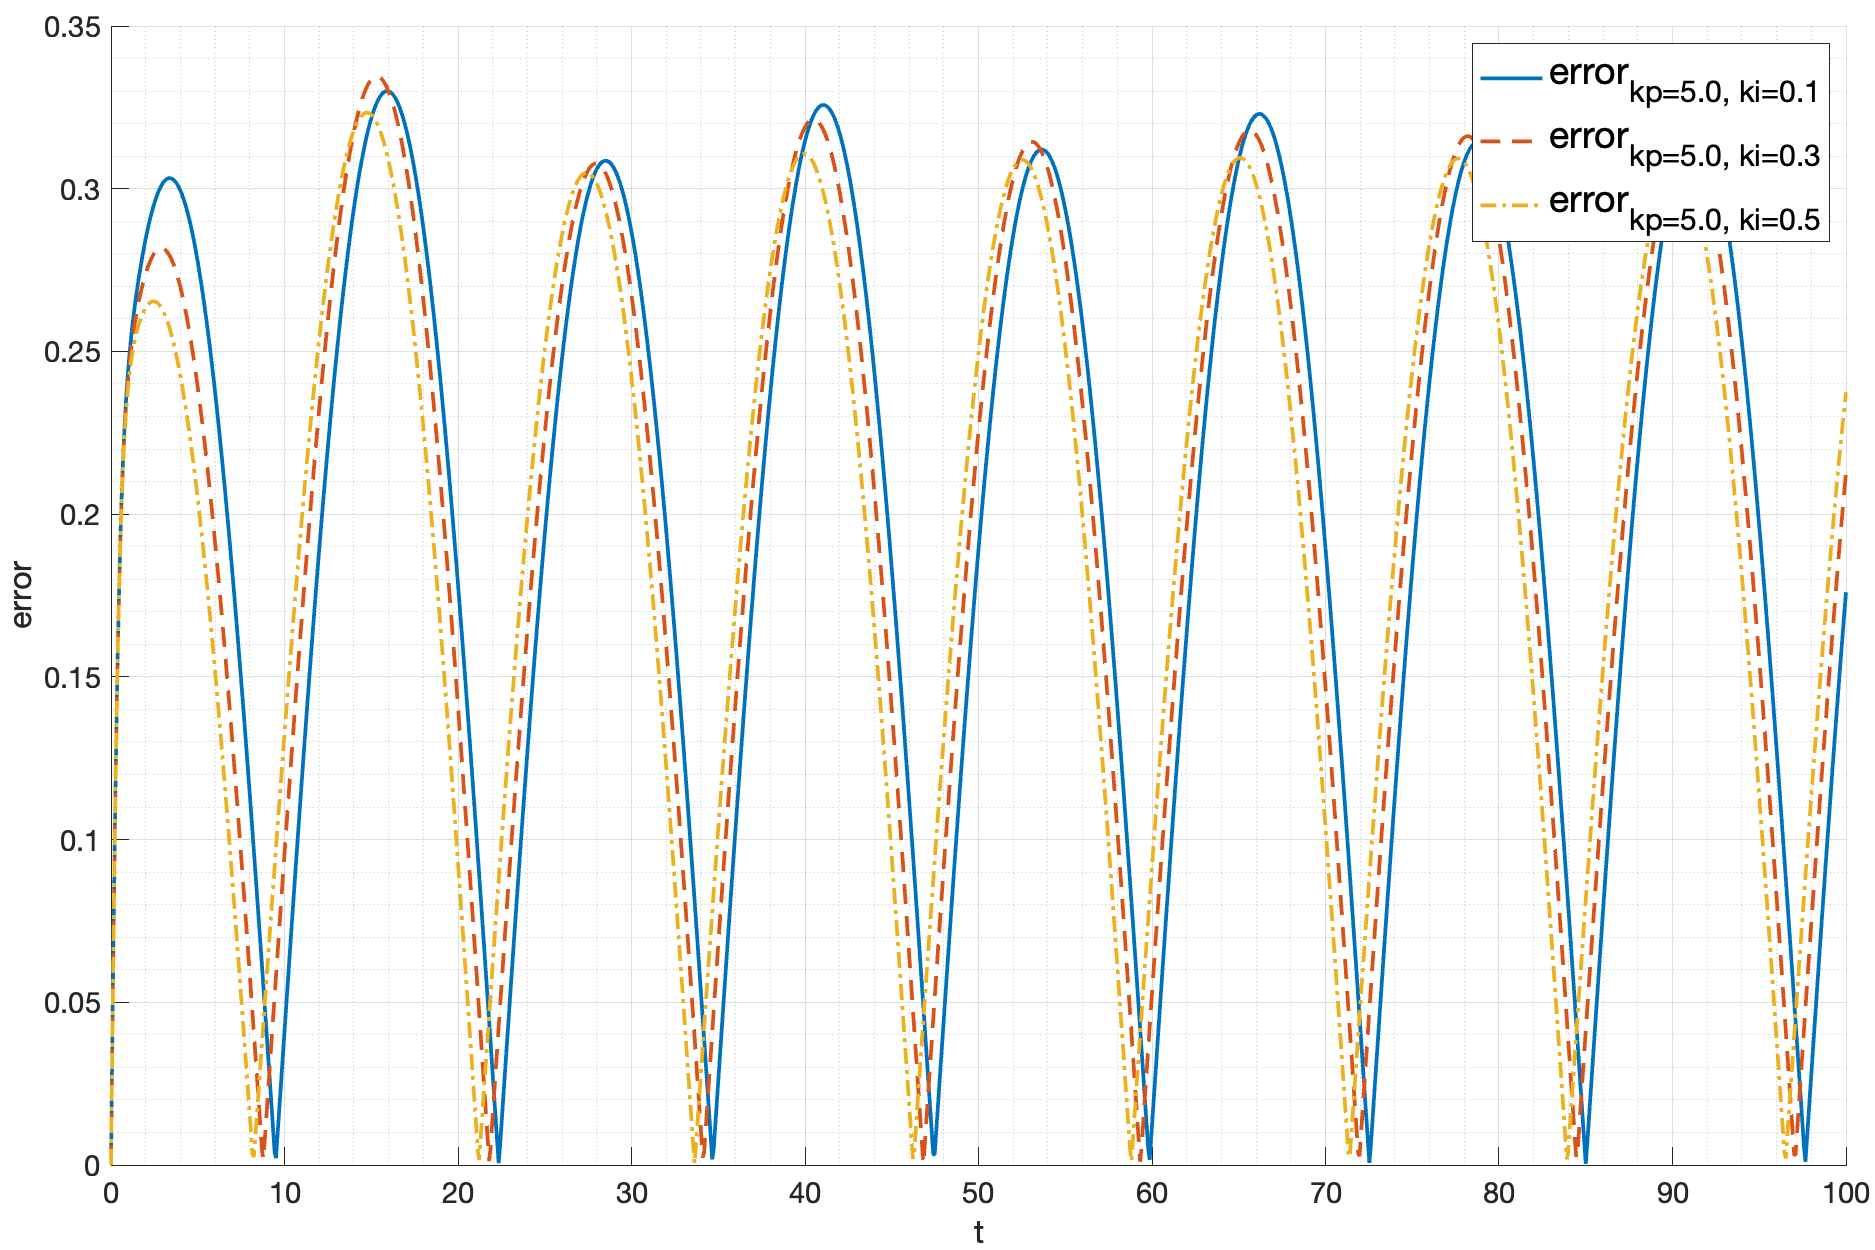
\includegraphics[width=\textwidth]{media/plots/task5_error_kp_5.0_2.png}
    \caption{График ошибки при $k_p = 5$}
    \label{fig:task5_error5}
\end{figure}

При $k_p = 10$ графики выходного сигнала и ошибки приведены
на рис. \ref{fig:task5_out6} и \ref{fig:task5_error6} соответственно.

\begin{figure}[ht!]
    \centering
    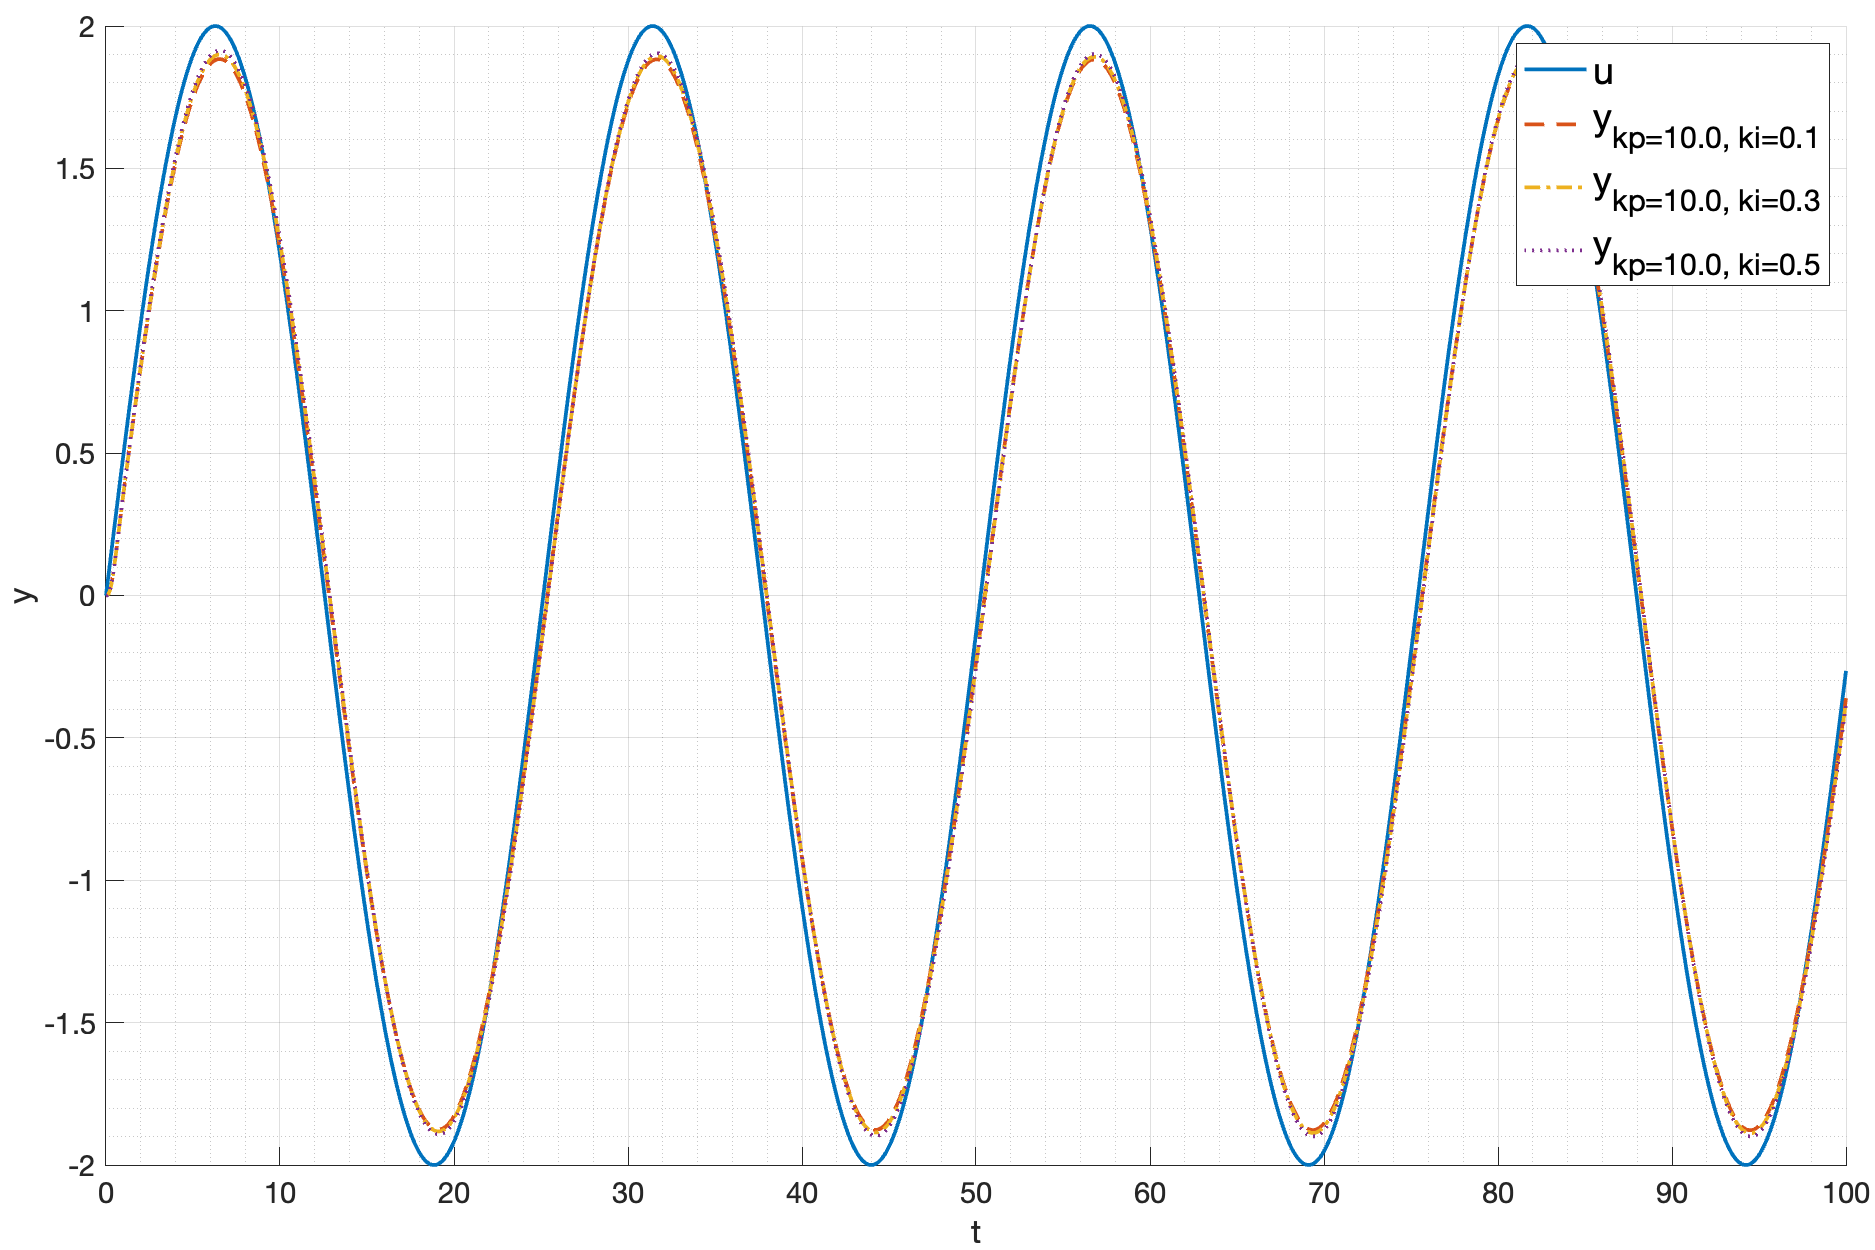
\includegraphics[width=\textwidth]{media/plots/task5_out_kp_10.0_2.png}
    \caption{График выходного сигнала при $k_p = 10$}
    \label{fig:task5_out6}
\end{figure}

\begin{figure}[ht!]
    \centering
    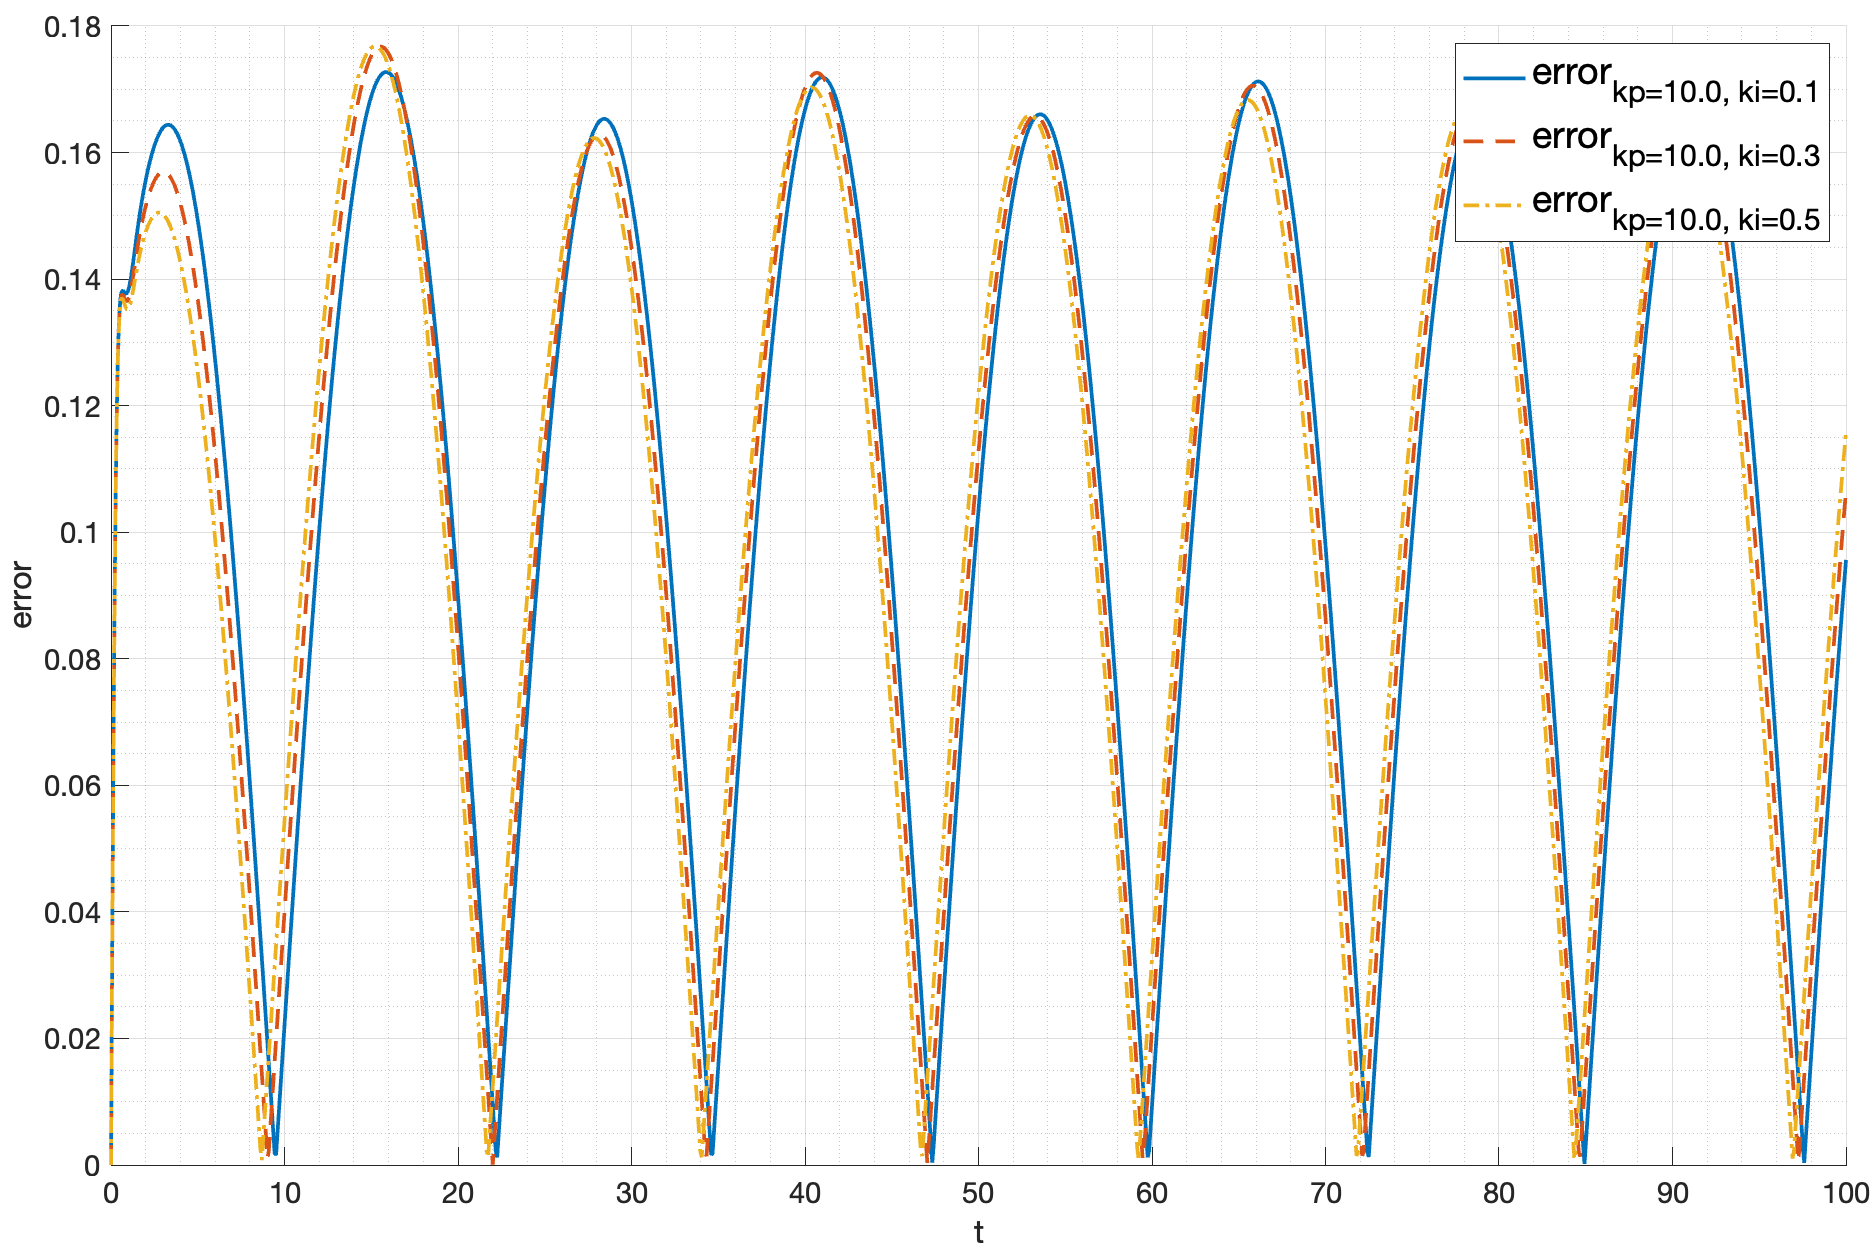
\includegraphics[width=\textwidth]{media/plots/task5_error_kp_10.0_2.png}
    \caption{График ошибки при $k_p = 10$}
    \label{fig:task5_error6}
\end{figure}

Видно, что при увеличении коэффициента $k_p$ уменьшается ошибка 
по фазе, при увеличении коэффициента $k_i$ уменьшается ошибка по амплитуде. 

\subsection{Вывод}

В данном разделе была рассмотрена система с астатизмом первого порядка и PI регулятором, 
влияние коэффициентов $k_p$ и $k_i$ на систему.
Можно сделать вывод, что коэффициенты $k_p$ и $k_i$ влияют на скорость сходимости системы и на величину ошибки.
Конкретный характер влияния зависит от вида входного воздействия, но в целом можно сказать, 
что при увеличении коэффициента $k_p$ система быстрее сходится к установившемуся значению,
при увеличении коэффициента $k_i$ уменьшается статическая ошибка. 
